\chapter{Supplementary materials for \autoref{chap:CMZ}}
\section{Description of the computational cluster used in the work}
\label{cluster}

\section{Developmental progression of naso-temporal population asymmetry in the CMZ}

\begin{figure}[!h]
    \makebox[\textwidth][c]{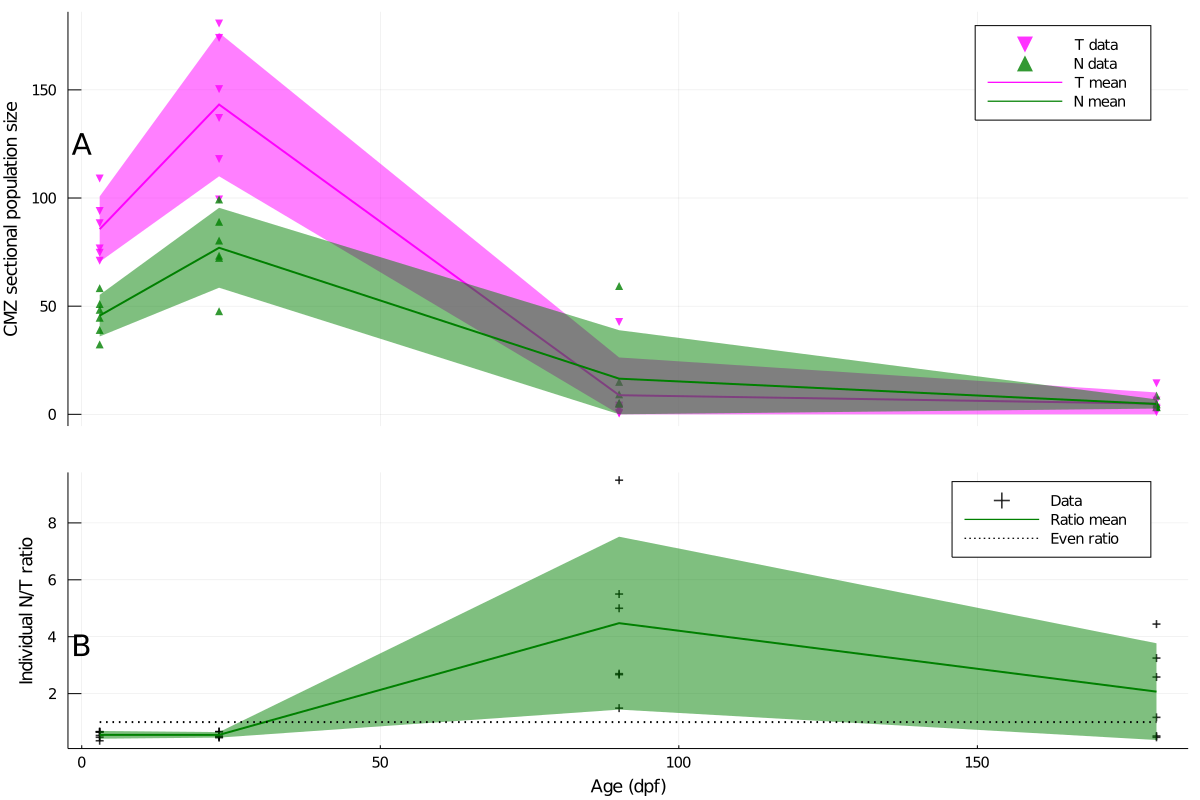
\includegraphics[width=1.2\textwidth]{cmz/NTontology.png}}    
    \caption{{\bf Developmental progression of naso-temporal population asymmetry in the CMZ.}}
    Marginal posterior distribution of mean nasal (N) and temporal (T) population size in 14$\mu$m transverse cryosections (panel A) or intra-individual N/T count asymmetry ratio (panel B), $\pm 95\%$ credible interval, n=6 animals per age. Data points represent mean counts from three central sections of an experimental animal's eye. 
    \label{NTontology}
\end{figure}

\FloatBarrier

\section{Cumulative EdU Bayesian Linear Regression}

\begin{figure}[!h]
    \makebox[\textwidth][c]{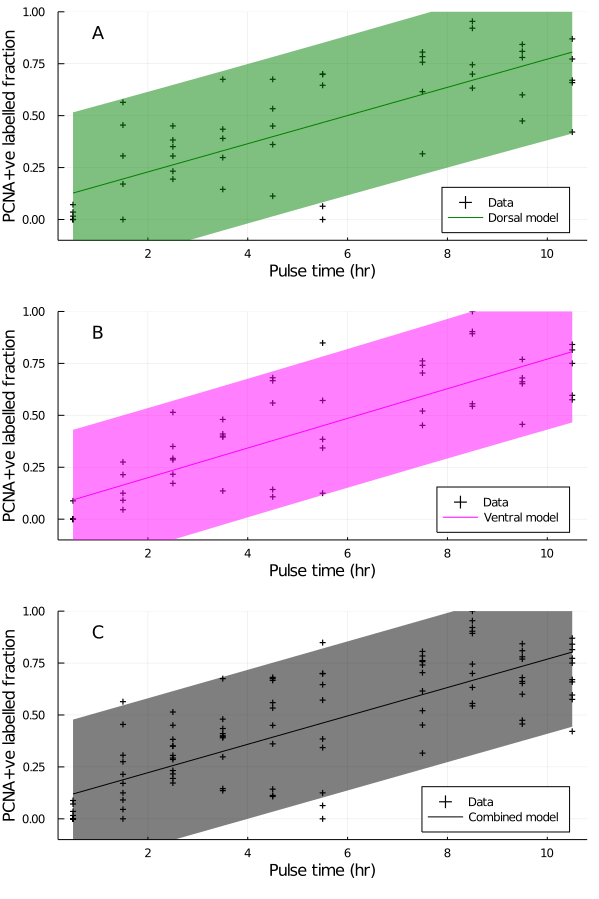
\includegraphics[width=.7\textwidth]{cmz/3ddvlinreg.png}}    
    \caption{{\bf Linear regressions performed on cumulative labelling data from dorsal, ventral, and combined CMZ sectional populations}}
    \label{cumEdUlinreg}
\end{figure}

\FloatBarrier

\section{Evidence calculations for Normal and Log-Normal models of layer and lineage contribution}

\begin{table}[!ht]
    \begin{tabular}{|l|l|l|l|l|l|l|} 
        \hline
        {\bf Layer} & {\bf Marker} & {\bf Cell type} & {\bf $\mathcal{N}$ logZ} & {\bf Log-$\mathcal{N}$ logZ} & {\bf logZR} & {\bf $\sigma$ sign.}\\ \hline \hline
        GCL & Cohort & All GCL cells & -189.0 ± 1.4 & -193.5 ± 1.9 & -4.5 ± 2.4 & -1.90\\ \hline \hline
        GCL & Isl2b & RGC & -74.5 ± 1.0 & -98.68 ± 0.24 & -24.2 ± 1.1 & -22.74\\ \hline
        GCL & Pax6 & Displaced am. & -101.93 ± 0.96 & -77.87 ± 0.27 & 24.06 ± 1.0 & 24.15\\ \hline
        GCL & Isl2b/Pax6 & RGC subtype & -97.9 ± 1.0 & -113.4 ± 0.74 & -15.5 ± 1.3 & -12.37\\ \hline \hline
        INL & Cohort & All INL cells & -184.0 ± 1.4 & -474.5 ± 2.7 & -290.4 ± 3.1 & -94.02\\ \hline \hline
        INL & Pax6 & Amacrine cell & -36.83 ± 0.88 & -65.43 ± 0.24 & -28.6 ± 0.92 & -31.25\\ \hline
        INL & PKC$\beta$ & Bipolar cell & -37.83 ± 0.2 & -0.77 ± 0.67 & 37.06 ± 0.7 & 53.12\\ \hline
        INL & GS & M\"{u}ller glia & -25.11 ± 0.2 & 6.7 ± 1.1 & 31.8 ± 1.1 & 29.22\\ \hline
        INL & HM & Horizontal cell & -31.97 ± 0.27 & 6.73 ± 0.61 & 38.7 ± 0.66 & 58.37\\ \hline \hline
        ONL & Cohort & All ONL cells & -201.0 ± 1.5 & -335.3 ± 1.5 & -134.2 ± 2.1 & -63.65\\ \hline \hline
        ONL & Zpr1 & Double cones & -93.7 ± 1.4 & -146.91 ± 0.8 & -53.2 ± 1.6 & -33.23\\ \hline
    \end{tabular}
   
    \begin{flushleft}logZ: logarithm of p(D), the marginal likelihood of the data, or model evidence.  Largest evidence values bolded. logZR: evidence ratio; positive values in favour of stable model.
    \end{flushleft}
    \label{lineage_nlnev}
\end{table}

\section{Likelihood ratio calculations for Normal and Log-Normal models of layer and lineage contribution}

\begin{table}[!ht]
    \begin{tabular}{|l|l|l|l|l|l|l|} 
        \hline
        {\bf Layer} & {\bf Marker} & {\bf Cell type} & {\bf $\mathcal{N}$ MLE} & {\bf Log-$\mathcal{N}$ MLE} & {\bf lhR}\\ \hline \hline
        GCL & Cohort & All GCL cells & 94.374 & 91.888 & -2.487\\ \hline \hline
        GCL & Isl2b & RGC & 8.265 & 7.403 & -0.862\\ \hline
        GCL & Pax6 & Displaced am. &  8.905 & 11.25 & 2.345\\ \hline
        GCL & Isl2b/Pax6 & RGC subtype & 14.464 & 15.248 & 0.784\\ \hline \hline
        INL & Cohort & All INL cells & 75.439 & 71.902 & -3.537\\ \hline \hline
        INL & Pax6 & Amacrine cell & 24.062 & 28.753 & 4.691\\ \hline
        INL & PKC$\beta$ & Bipolar cell & 38.285 & 40.184 & 1.899\\ \hline
        INL & GS & M\"{u}ller glia & 45.279 & 49.521 & 4.242\\ \hline
        INL & HM & Horizontal cell & 43.817 & 46.461 & 2.645\\ \hline \hline
        ONL & Cohort & All ONL cells & 65.658 & 69.605 & 3.947\\ \hline \hline
        ONL & Zpr1 & Double cones & 11.934 & 12.782 & 0.848\\ \hline
    \end{tabular}
   
    \begin{flushleft}logZ: logarithm of p(D), the marginal likelihood of the data, or model evidence.  Largest evidence values bolded. logZR: evidence ratio; positive values in favour of stable model.
    \end{flushleft}
    \label{lineage_lhratio}
\end{table}


\section{Methods}
\label{ssec:CMZmethods}

\subsection{Statistical Analyses}


